\documentclass[double,12pt]{beavtex}
\title{Visualizing Contribution Patterns in Open Source}
\author{Rithika Kiran Naik}
\degree{Master of Science}
\doctype{THESIS}
\department{Electrical Engineering and Computer Science}
\depttype{School}
\depthead{Director}
\major{Computer Science}
\advisor{Carlos Jensen}
\submitdate{September 17, 2015}
\commencementyear{2016}
\usepackage{graphicx}
\usepackage{caption}
\usepackage{float}
\restylefloat{table}
\usepackage[toc,page]{appendix}
\usepackage{dirtytalk}
\graphicspath{ {images/} }



\abstract{Open Source software gives users the freedom to copy, modify and redistribute source code without legal entanglements. The evolution of these software communities usually depend a lot on how the participating developers and users interact and co-operate with each other. Over the past few years, open source software have become widely accepted and used, hence making the study of their organization and sustainability a very hot topic. To understand the working philosophy, health, and evolution of any open source project, one needs to look at a variety of factors like community interaction, strength of connections, recruiting and mortality, support and contribution patterns. Getting, sharing and analyzing Software Development metrics and information related to open source projects has thus become important, with many projects and companies looking to do so. The main challenge however is distilling large amounts of data into actionable intelligence. The main idea behind this work is to help communities and others understand contribution patterns in open source projects through the use of various visualization techniques. }

\acknowledgements{I would like to take this opportunity to thank my advisor, Dr Carlos Jensen, for his patience and constant support throughout the phase of this research. All the brainstorming sessions to discuss every minute detail in progress were extremely fruitful. My sincere gratitude to Dr Anita Sarma, Dr Cindy Grimm, Dr Kathy Mullet for accepting my invitation and taking time to be a part of my Graduate committee. 

My gratitude to team Bitergia as this work would not have been possible if not for their quest to learn more. So thank you Jesus M  Gonzalez Barahona and Gregorio Robles for providing me with the necessary datasets and valuable suggestions.

Thank you Jennifer Davidson, Shankar Jothi and Subarna Kar for all the help during the course of this work and all my friends in Corvallis for the wonderful 2 years away from home. Special thanks to the entire Human Computer Interaction group for looking through my work and providing me with timely inputs.

My dream of pursuing a Master's degree would not have been fulfilled if not for my parents constant encouragement and faith in me. Thank you Mom and Dad for everything !
}

\begin{document}

\maketitle

\mainmatter

\chapter{Introduction}
The software industry has undergone a lot of changes over the years and one such important change was the advent of Open Source Software(OSS). Open source software is a type of software whose development  is volunteer driven \cite{ghosh2005} and for which the code base is made available for any person to modify, edit and redistribute \cite{osdef}. Open source software is being heavily relied on and used today because of-
\begin{enumerate}
\item Quality: Research has found support for the saying that in Open Source, \say{Given enough eyeballs, all bugs are shallow} \cite{linuslaw}. Furthermore, by being developed by a large and diverse base of developer teams, applications also develop a large variety of features, huge support groups and overall enhanced products \cite{pcwr}. 
\item Flexibility: Open Source gives users the ability to tweak any part of the functionality to match their needs \cite{pcwr}. 
\item Auditability: Access to the code base promotes transparency around issues like security, freedom, flexibility etc., something lacking in closed source
software \cite{pcwr}. 
\item Large support base: Available in the form of documentation, forums, mailing lists, forges, wiki, live chats and so on and with so many options available a user can never hold onto a problem long enough. 
\end{enumerate}
With a plethora of such important features and advantages, the adoption of Open Source has been steadily increasing. 

Managing any software development effort comes with its own set of challenges and OSS is no different. Having mentioned its advantages, managing these distributed communities is a big task. With the code base made available to all, issues like maintaining coding standards, peer review processes, skill sets, documentation etc. are important \cite{tum2005}. The fact that these efforts are volunteer based brings up issues of fairness and equity among the developers. OSS relies heavily on its community for its growth and development \cite{seth2010}, making co-ordination among them a foremost point of importance. The OSS communities usually have a lot of developers from all over the world who volunteer to produce code and support the software in general. Their motivations have been open to studies \cite{greg2002}. Unlike traditional software, OSS has a wide spread developer/volunteer group, the success or failure depends strongly on its community, as they can make or break the project. The onion model divides the developer lifecycle into 7 layers, with each layer moving inwards, showing the level of involvement of the developers. The outermost layer is considered as the starting point for a new developer after which they slowly transition to higher points of responsibilities, if they continue to stay with the organization, with the final stage being, becoming a part of the core community and a regular contributor \cite{kishida2003}.

\begin{figure}[H]
\centering
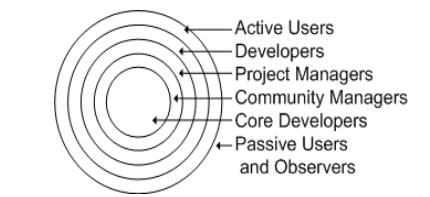
\includegraphics[width=90mm]{onion.png}
\caption{Onion model by Ye and Kishida}
\end{figure}

This being the basis to understand a developer's growth, how can one know the spread of the developers who contribute? Current approaches rely on very biased or incomplete knowledge bases, for instance, finding a large of number of developers joining the project and marking that to be as a growing project \cite{igor2014}. As the community benefits by having developers from all across the world, it is important to identify the regions which contribute more to the open source world and the regions which need help. This can help researchers identify why developers in a certain regions contribute more or less than others. This was the first motivation for this research. Also, a project's peak phase of success can be noted by looking at the community size and contribution size at any given time. This can then be probably used to predict future structure of the communities for the projects. This became the second motivation.


\section{Why Data Visualizations?}
In 1973, the Anscombe's Quartet showed how four sets with nearly identical statistical properties, appeared very different when graphed \cite{wiki}. This led to the thought that understanding data by just looking at it might not necessarily be useful or correct. Hence visualizations have gained a lot of importance as tools to promote understanding. As the proverb says,"A picture is worth a 1000 words", visualizations throw light on datasets in a completely new way. As the amount of data increases, finding a common way of unifying the data with the its underlying meaning is needed. Comparing, contrasting, reviewing data becomes easier when one views various visualizations. Besides creating visualizations, it is necessary to understand the requirement in hand, perform data manipulation accordingly and then create a suitable visual diagram. Failing to differentiate between excess data and useful data would result in unfavorable results during visualization analysis.
The main goal here was therefore to build a neat, easily accessible, intuitive and effective set of visual interfaces which can give an insight on the trends in open source projects with regard to developer's contributions and experiences.


\chapter{Related Work}
Researchers all over the world have performed different types of studies, surveys, observations etc. on the trends in open source projects. They are continuously looking at the open source communities and contributor motivations to get a grasp on how the open source communities function to be sustainable. For this reason the Linux Foundation releases a yearly survey to understand how they performed and looks at various variables ranging from code quality, to the size and composition of the developer base, to support issues and their preferred way of showing these varied results are through visualizations \cite{lfs}. This has become a guideline for most surveys today as it holds a lot of information that would help understand the growth of an open source community. Surveys have been conducted with around 1600+ developers all over the world to look at areas like developer role in open source projects, extent and intensity of open source contributions, support coming in from the core team. The surveys have also showed some demographic data like male to female ratio, employment status, living area, formal education level, reasons to contribute to an open source project etc \cite{david2003}. But the survey just gave a general overview of developers contributing and made no emphasis beyond that. Another interesting area looked at to understand a developer's motivation was to understand how their roles affected the evolution of the community. Ye and Kishida looked into these motivation factors and stated, \say{Learning plays a big part in getting developers to contribute} \cite{kishida2003}. This was seconded by the study to understand the development in Apache and Mozilla, where they also found that learning and capability to solve a problem are major motivations for developers at any level in an open source project \cite{mockus2002}. A lot of research has been done to understand developer motivations in open source and sustainability factors like number of developers in a project \cite{david2003, rishab2002}, size and quality of the code base \cite{marc2014}, number of users for any given project \cite{rishab2002}, functioning principle of projects \cite{tarja2013}, etc. Also the evolution of open source projects were keenly looked upon by looking at methodology, code sets, tool sets, performance evaluation, maintainability, social network growth of developers and many such attributes that have an impact on a community \cite{tarja2013}. 

In 2014, research was done to gauge the health of an open source community. This work was done by tools prepared to gauge certain communities or platforms, and were not universal
in nature. For example, specific solutions existed for communities like GNOME \cite{gno}, Debian \cite{ver2011} etc., accessing the data repositories, but the same tools could not be used for other communities \cite{gno}. There were frameworks that monitor and analyse repositories that were more generic, but still had their own limitations with technologies \cite{marc2014}. This research made use of service oriented computing monitoring techniques to gauge the health of an open source community by being as generic as possible and looked into the code base and activity revolving around it \cite{marc2014}. 

The most common factor found by researchers while gauging the health and evolution of OSS was the impact the communities had on the projects. It might be possible that a sustainable community could be attained with a constant inflow of developers with varied skill sets, ages and from a geographically wide area. This might also go onto show a wide spread knowledge about the project and a good mix of ideas and interests. 


\section{Experience of Developers}
In 2002, a study was conducted on two open source projects, Apache and Mozilla. One of the parameters that was looked at was developer participation, where they looked at the frequency of contributions over a period of time. They concluded that, in Apache and Mozilla at least, the core group was highly active and apart from them, only a handful of developers, not in the core group contributed on a regular basis \cite{mockus2002}. The researchers at Notre Dame University studied the parameter on a larger set of open source projects, and noted that developers in open source projects are not as well connected as developers in other collaborative networks \cite{greg2002}. 
In an article in 2014 \cite{jes2014}, researcher Jesus Barahona stated, \say{In order to gauge a community's health it is important to keep track of the developer ages}. He points out that attracting new developers is important, but retaining the experienced ones also was a high priority. The ratio of experienced, long term members to recent ones has a high impact on the quality of code and the ability to support members \cite{jes2014}.

\textbf{Turnover:}
Shows how people are entering and leaving the community. An indication of the community's attractiveness and stability.

\textbf{Age:}
Measures how long ago each current member joined a project. An indication of how many people are at what stage of experience, from old-timers to newbies.

Together these metrics can be used to estimate engagement, to predict the future structure and size of the community, and to detect early potential problems that could prevent the healthy growth of a project \cite{jes2014}.

\section{Geographic Diversity of Developers}
It is interesting to note that although studies have been conducted to understand the motivations of the developers, understanding the range of developers contributing, geographically or age wise, is still very crude. Greogorio Robles and Gonzalez-Barahona were among the first ones to look into the geographic factors that influenced developer contributions \cite{kishida2003}. They collected data of all the registered users from SourceForge, the largest libre software web based platform which had data about geographic locations. They came up with a distribution of developers in different regions of the world. The result of this study showed North America in the forefront with the highest number of contributors, followed by Europe and clusters of Asia, Australia, South America and Africa \cite{robles2006}. The problem here was that the information about location or geography was not captured cleanly in SourceForge. It was mostly left blank during account creation by the account holders.  
After this came the study by Takhteyev Y, Hilts A and they studied open source data made available by Github, which was becoming a pioneering source management application. But there were problems here as well as the dataset was either incomplete or was not categorizable by Top Level Domains(TLD) \cite{yuri2010}. Then came the idea of looking at time zones and Internet Protocols(IP) of the systems of the users who contribute, both collected through SourceForge \cite{von2010}. But the issue with looking at IP addresses was that the dataset was not available to all and agreements needed to be signed for the same \cite{von2010}. Results from the above mentioned studies all show that European and North American countries particularly Unites States of America were the major areas where developers were mostly located and worked from \cite{yuri2010, von2010}. A survey by Ghosh et al \cite{ghosh2005} showed the influence of French, American and German developers but the survey that was conducted by Tuomi et al \cite{tuomi2004} showed varied results leaning a lot towards US, UK, Canada and Germany.

\chapter{Data Gathering and Processing}
Bitergia was founded by four professors from the Universidad Rey Juan Carlos, Spain in July 2012 \cite{bit}, trying to further our understanding of the open source community and its growth. The focus was to develop data analytic techniques to mine information about project performance, track developer actions, and areas of improvement and identify risks involved in
further development.

I leverage the tools and techniques they developed, in my thesis, adding novel visualizations of the data they generate.

\section{Services provided}
They built tools to extract data from repositories like SVN and Git, from mailing lists, from bug trackers like Jira, Bugzilla, Allura etc. These tools together are known as the \emph{MetricsGrimoire Library} which is accessible to all in Github \cite{metrics}.

\begin{figure}[H]
\centering
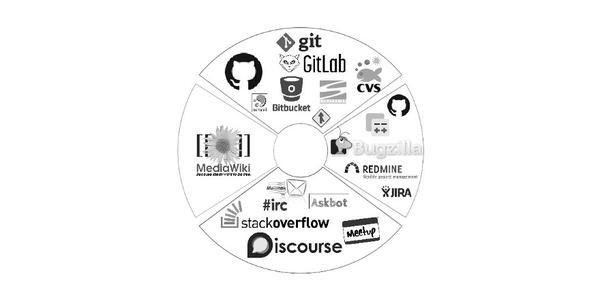
\includegraphics[width=140mm]{bitergia.jpg}
\caption{Bitergia data forums}
\end{figure}

With the tools ready to extract data, the next step was to build a framework which would help them analyze and visualize the data obtained from the Metrics-Grimoire tools. This is known as the \emph{VizGrimoire Library}. With such a vast tool base available, it became a lot easier to extract the necessary data for my projects. The dashboards made by Bitergia have been highly acclaimed and used by organizations like Apache, Eclipse, Puppet Labs etc which only added to their credibility.


\begin{figure}[H]
\centering
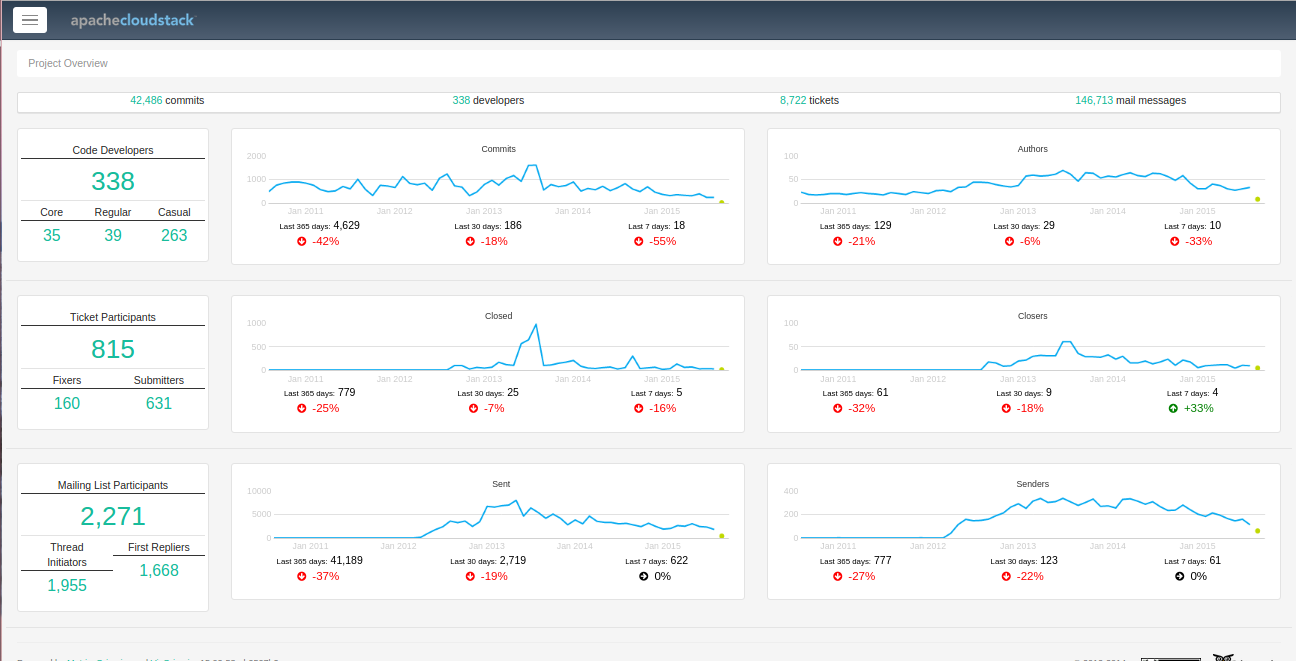
\includegraphics[width=120mm]{apache.png}
\caption{Apache Cloudstack Dashboard}
\end{figure}

\begin{figure}[H]
\centering
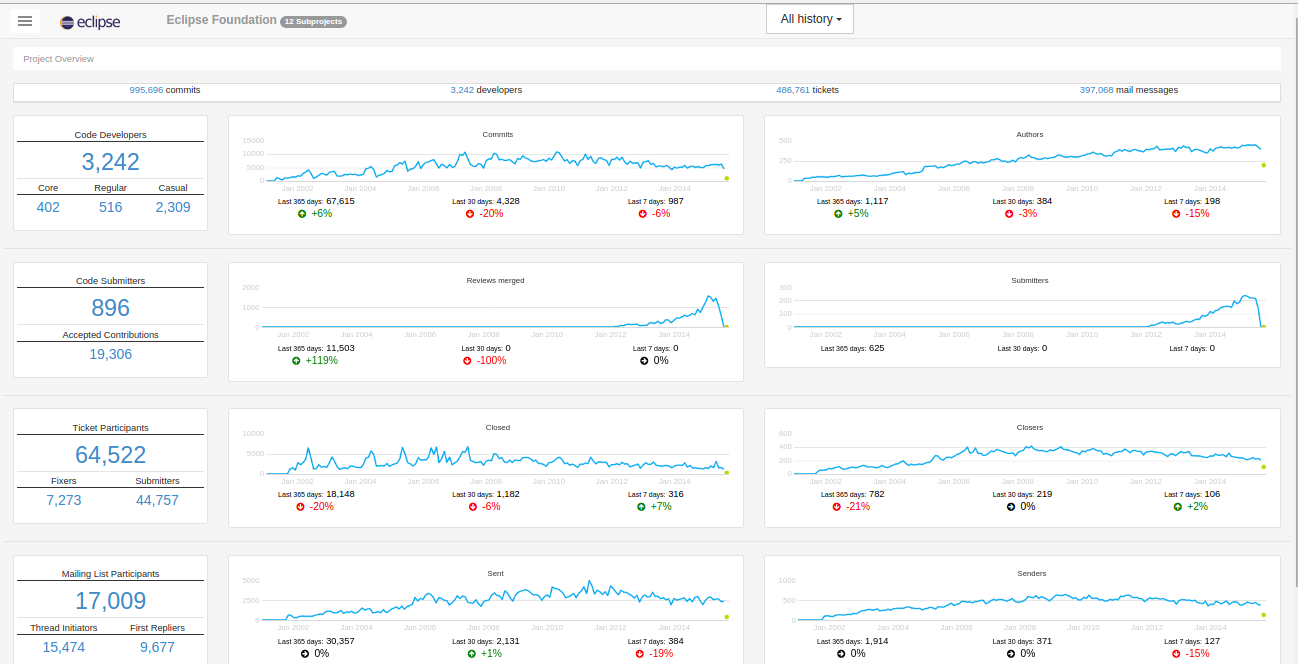
\includegraphics[width=120mm]{eclipse.png}
\caption{Eclipse Dashboard}
\end{figure}

\section{Task at hand}
Bitergia had some basic implementations done for the two cases previously explored. 

\textbf{CASE 1 - Experience of Developers}

The Bitergia team focused on calculating age in project for active developers at a given time. As a result of their work the following visualizations were built-

\begin{figure}[!ht]
\centering
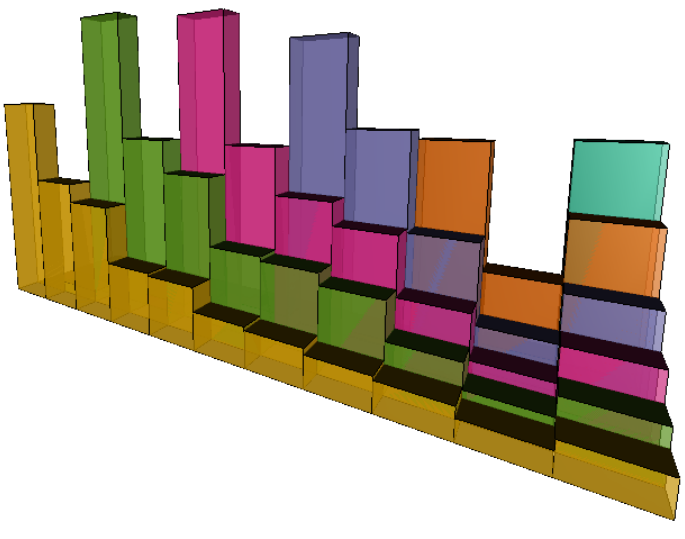
\includegraphics[width=90mm]{age2.png}
\caption{3D version of pyramids every two years. The height of each bar depicts the number of developers that stayed for 'x' number of years and each color depicts the data for a particular year.}
\end{figure}

\begin{figure}[!ht]
\centering
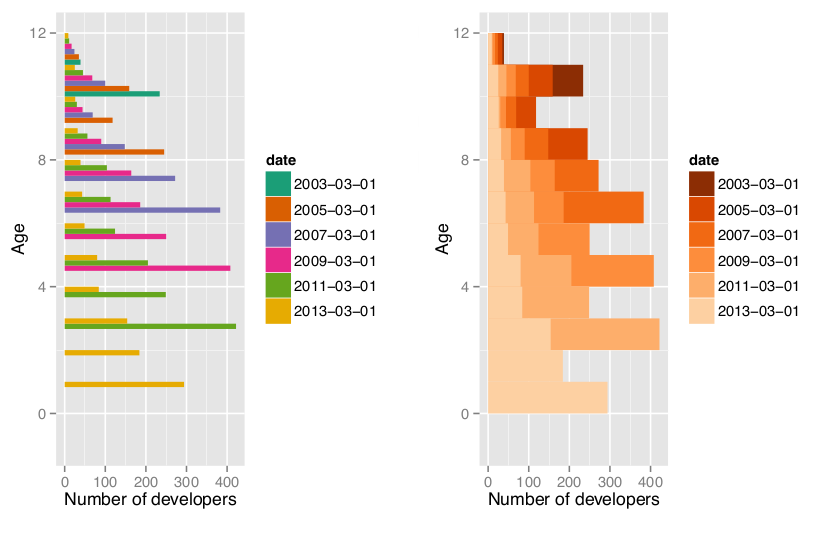
\includegraphics[width=130mm]{age1.png}
\caption{Comparison for pyramids every two years. The colors here point to data from the corresponding years and the height of the bar is the measure of the number of developers in each quarter.}
\end{figure}

3D visualizations are generally deemed to be difficult to understand due to their structuring and also a user would need to view them from different orientations which adds to the complexity \cite{james2011}. This could have led to difficulty in understanding the visualization. 

 \textbf{CASE 2 -Where do Developers work ?}

Location has always been of prime importance in any area of work. In the software industry, distance has never been a matter of concern because of the nature of work involved, with this being even more true for OSS as its developers are assumed to be contributing according to their convenience \cite{yuri2010}. Bitergia’s main source of data for this was collected from
Github and mailing lists. Because most projects hide developers full email addresses and IP addresses, certain assumptions had to be made, and geography had to be determined by time zones. They came up with two basic visualizations.

\begin{figure}[!ht]
\centering
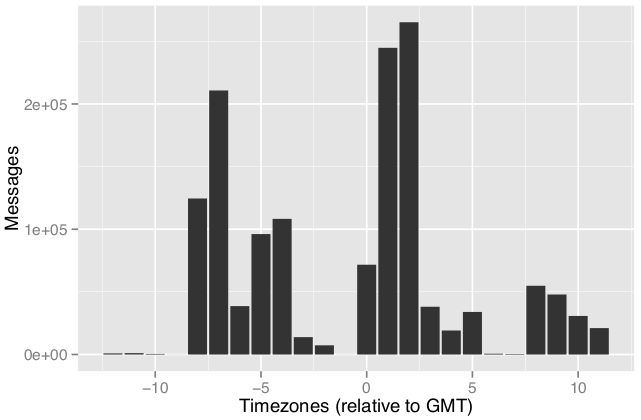
\includegraphics[width=90mm]{work1.png}
\caption{Time zone origin of messages}
\end{figure}

\begin{figure}[!ht]
\centering
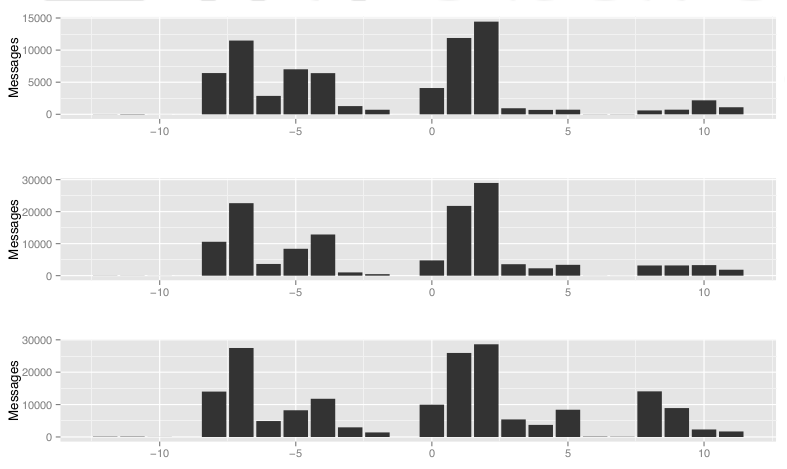
\includegraphics[width=90mm]{work2.png}
\caption{Time zone origin of messages for 2002,2007,2012}
\end{figure}

The following was the division of geography with respect to time zone -

1. America: GMT-8 to GMT-2 (US/Canada: -8 to -4)

2. Europe/Africa/Middle East: GMT to GMT+5

3. East Asia/Australia: GMT+8 to GMT+11


The basic nature of the visualizations didn't help provide a lot of detailed understanding about the developer distribution for an organization. They were more oriented to giving an
overview of messages per time zone. The relation between commits and authors and location was not clear and needed more than a birds' eye view type of a visualization.

\chapter{Methodology}
To help explore the previously explained cases, we looked into improvising the provided visualizations to help people understand the data in a better way. To carry out this process, datasets for 5 open source projects were collected. Different prototypes were implemented for each case and improved through informal formative evaluations with the research team. Initial visualizations were built and an iterative process of development was followed.

\section{The Organizations}
\begin{enumerate}
\item Eclipse Foundation :
This is a member supported open source community focused on building a platform comprised of extensible frameworks, tools and runtimes for building, deploying and managing softwares across the lifecycle \cite{eclipse}.
\item OpenStack :
It is one of the most active open source products currently available for all types of cloud environments. It controls a large number of resources for computation, storage ,networking for a datacenter \cite{openstack}.
\item Puppet Labs :
This is an open source tool which manages various stages of IT infrastructure inclusive of provisioning, patching, configuration and management of operating systems across cloud structures \cite{puppet}.
\item RedHat RDO:
This is a community of people who are interested to use and deploy OpenStack on the RedHat Linux, Fedora distributions. It is a sub community of people who use RedHat which is one of the largest contributors to Linux \cite{rdo}.
\item Citrix Apache Cloudstack :
This is an OSS which deploys and manages networks of virtual machines as a IaaS(Infrastructure as a Service) platform. It supports VMware, KVM, XenServer, Hyper-V \cite{apache}.
\end{enumerate}

\section{Why the 5 projects?}
The choice of projects were driven by a desire to cover a variety of projects. In the selected 5 projects, the Eclipse Foundation and RedHat have been around and successful for a while now.
These projects also have a large developer community. OpenStack, Puppet Labs and Apache Cloudstack are relatively newer projects gaining popularity among the community. OpenStack has made its presence felt as cloud based software gathering a lot of buzz. Citrix's Apache Cloudstack was set up as a result of the gaining popularity of OpenStack, to help people using OpenStack on Linux. This gives us a set of projects with growing communities.

\section{Dataset}
Using the tools built by Bitergia, data for the 5 organizations were extracted. The files were all in the json format. All the data collected was till February, 2015 and
holds data from 2010 to 2015. The time zone files have data from time zone -12 to +11. One important field added to the time zone files, was the approximate population for each of the time zones which was taken from the below graph.

\begin{figure}[!ht]
\centering
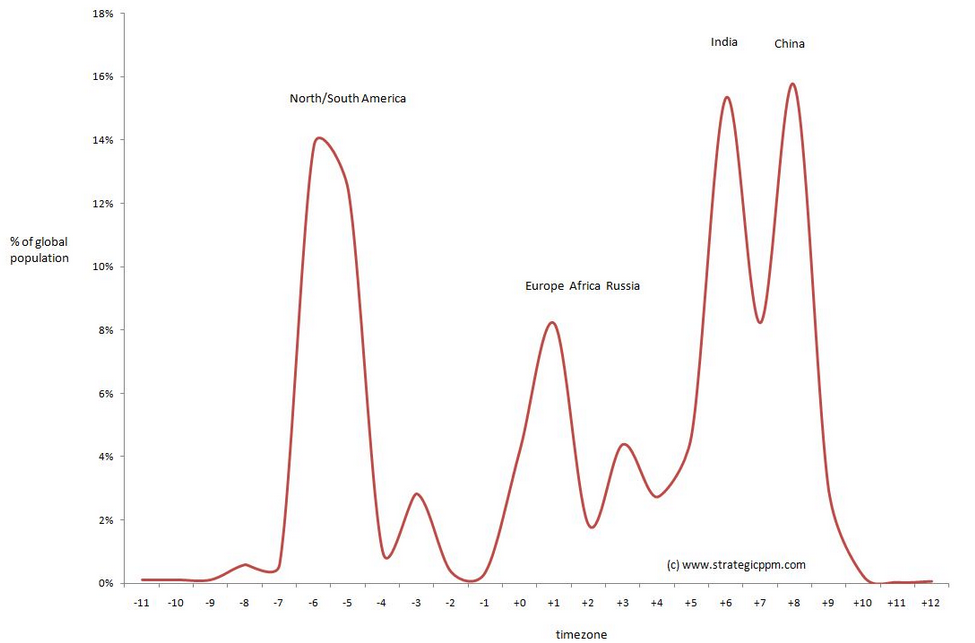
\includegraphics[width=160mm, height=100mm]{pop1.png}
\caption{Global population by time zone}
\end{figure}

Also in order to build a time zone based visualization, a geojson file was needed which would draw the map, time zone wise and this file was made available by a researcher on Techslides \cite{tech}. As geojson files have large overhead and would take a lot of time to load, converting it to topojson format was recommended \cite{tech}. Topojson is a command line application which not only reduces the size of geojson files, it also gives multiple options like simplification, conversion etc. It can be installed easily using Node Package Manager (NPM). 

The task was then to categorize the developers into different sections to find how many of them stayed for what intervals of time. A pattern was then searched for, to see if the joining
and leaving rates were consistent or showed any anomalies. The json files were modified to find these generation ranges.


\section{D3.js}
As the visualizations needed flexibility the most ideal tool in hand was D3.js \cite{d3}. D3 is a javascript library built by Mike Bostock which has the capacity to build
interactive, dynamic and a big variety of visualizations. It is largely based on HTML5, CSS and SVG. Due to the large developer support available for the library, it was an ideal choice to build the visualizations. It accepts external data in the form of json, CSV or TSV. Being a javascript library, it follows the same syntax, thus making data manipulation quick. This library is widely used by big corporates like Datameer, The New York Times, OpenStreetMap etc.

\section{Experimental Designs}

\subsection{Bitergia's Implementations}
The implementations done by team Bitergia are viewed to analyse the data set in hand. Figure \ref{fig:devExp} is used to show the experience of developers and is a bar chart. The y axis is age in quarters showing the duration that a developer stayed/contributed to the project and the x axis is the number of developers.

\begin{figure}[H]
\begin{center}
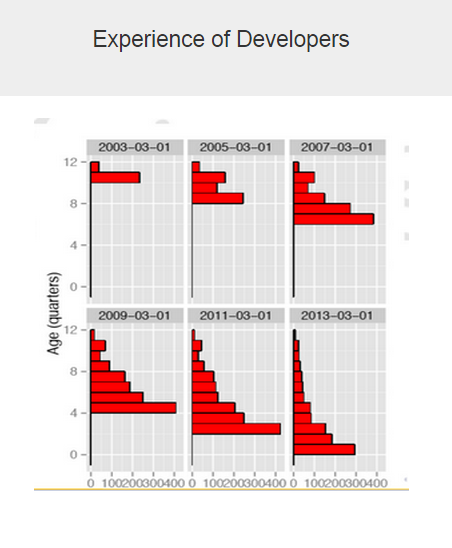
\includegraphics[width=90mm]{image11.PNG}
\end{center}
\caption{Experience of Developers}
\label{fig:devExp}
\end{figure}

Figure \ref{fig:devWork} is used to view the number of messages incoming from different time zones. The y axis is number of messages and the x axis is the time zones of the world. These two implementations were created out of the same datasets that were used for our implementations.

\begin{figure}[H]
\begin{center}
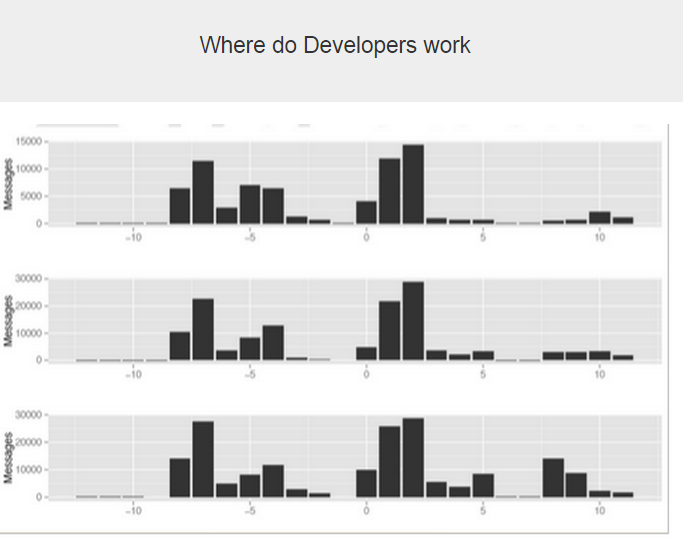
\includegraphics[width=90mm]{image12.PNG}
\end{center}
\caption{Where do Developers Work?}
\label{fig:devWork}
\end{figure}

\subsection{Our Implementations}
Figure \ref{fig:devTurn} is a grouped bar chart which has two main data sets - one column shows the number of developers who join the project each year i.e., New developers and the second column shows the number of developers that are still a part of the project each year i.e., Established developers.

\begin{figure}[H]
\centering
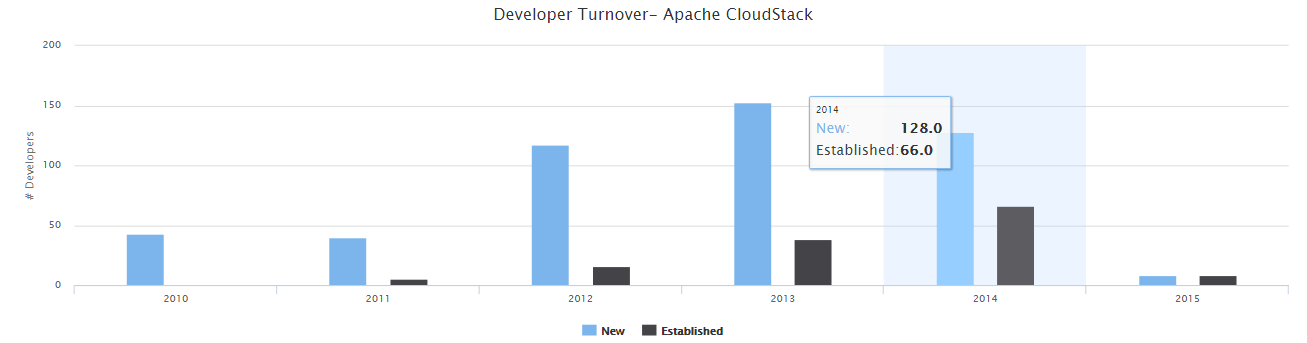
\includegraphics[width=130mm,height=60mm]{image1.PNG}
\caption{Developer Turnover}
\label{fig:devTurn}
\end{figure}

Figure \ref{fig:actAuth} is a stacked bar chart which gives an individual, a total look at the number of developers that are still active in a project over the years.

\begin{figure}[H]
\centering
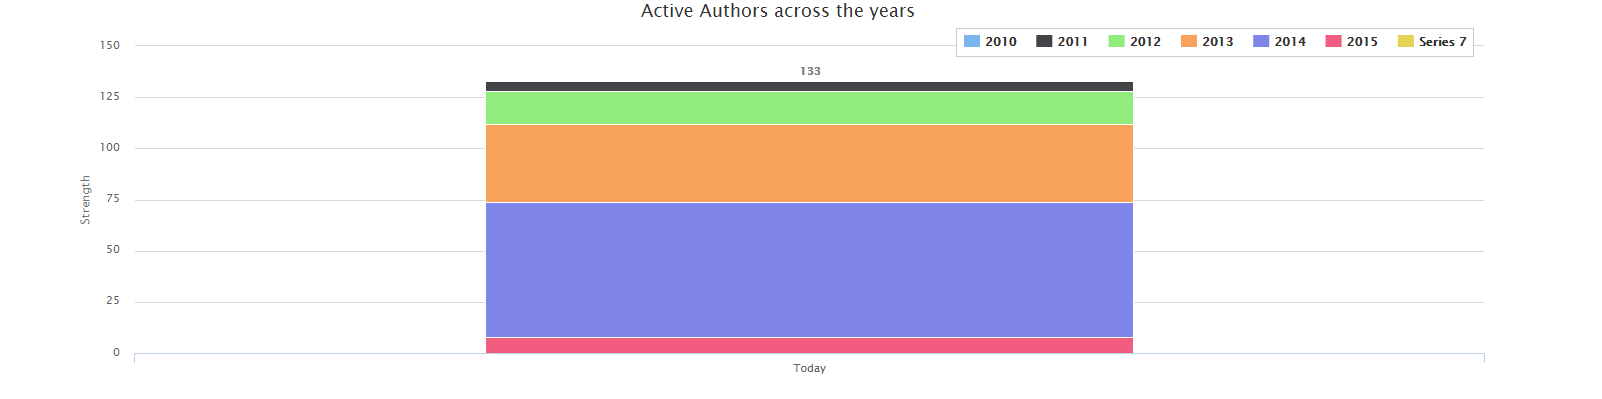
\includegraphics[width=170mm,height=70mm]{image2.PNG}
\caption{Active Authors Across the Years}
\label{fig:actAuth}
\end{figure}

Figure \ref{fig:devMort} is a also a stacked chart which shows the conversion rate i.e., percentage of developers that stay back in a project each year and the mortality rate i.e., percentage of developers that leave the project each year.

\begin{figure}[H]
\centering
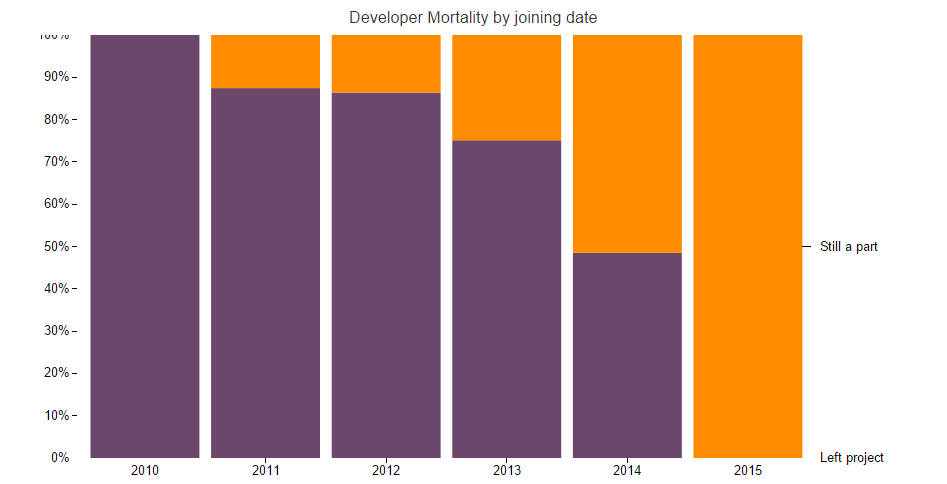
\includegraphics[width=130mm,height=60mm]{image3.PNG}
\caption{Developer Mortality by Joining Date}
\label{fig:devMort}
\end{figure}

From Figure \ref{fig:auHub} to Figure \ref{fig:div3} are all map based visualizations which use color as a main encoding mechanism to show one parameter from the dataset (population density). Figure \ref{fig:auHub} is colored according to the number of Authors present in each time zone according to the data from GitHub. Similarly Figure \ref{fig:auML} is shaded with the same parameter but using data taken from the mailing lists. In each of the figures below, the orange shaded countries had no data to available. This happened with countries which had \say{half time zones}, like India, central Australia, Iran, Myanmar, Nepal and a small part of Canada. Also data for countries lying in time zone +12 like Russia and New Zealand was not available either.

\begin{figure}[H]
\centering
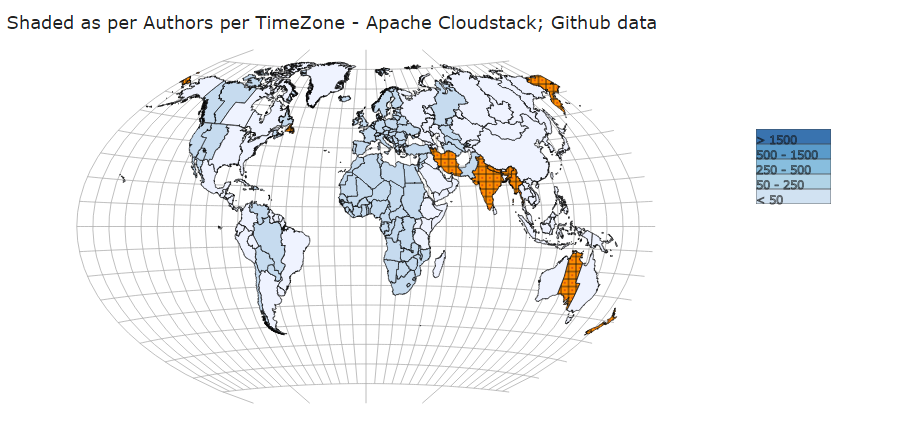
\includegraphics[width=130mm,height=60mm]{image4.PNG}
\caption{Authors per time zone - Github}
\label{fig:auHub}
\end{figure}

\begin{figure}[H]
\centering
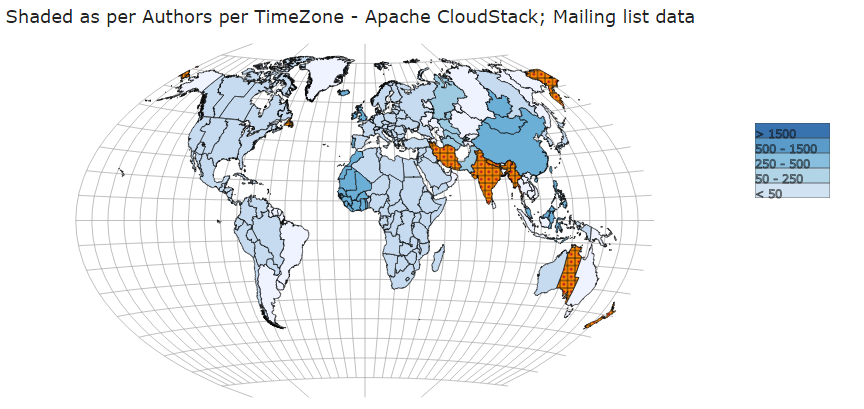
\includegraphics[width=130mm,height=60mm]{image5.PNG}
\caption{Authors per time zone - Mailing lists}
\label{fig:auML}
\end{figure}

Figure \ref{fig:coHub} and Figure \ref{fig:mgML} are shaded as per commits per time zone, data taken from both Github and Mailing lists.

\begin{figure}[H]
\centering
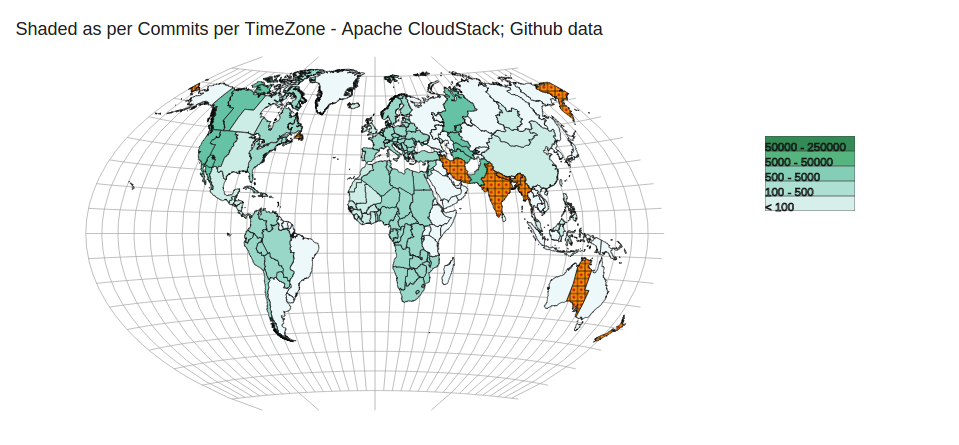
\includegraphics[width=130mm,height=60mm]{image6.png}
\caption{Commits per time zone - Github}
\label{fig:coHub}
\end{figure}

\begin{figure}[H]
\centering
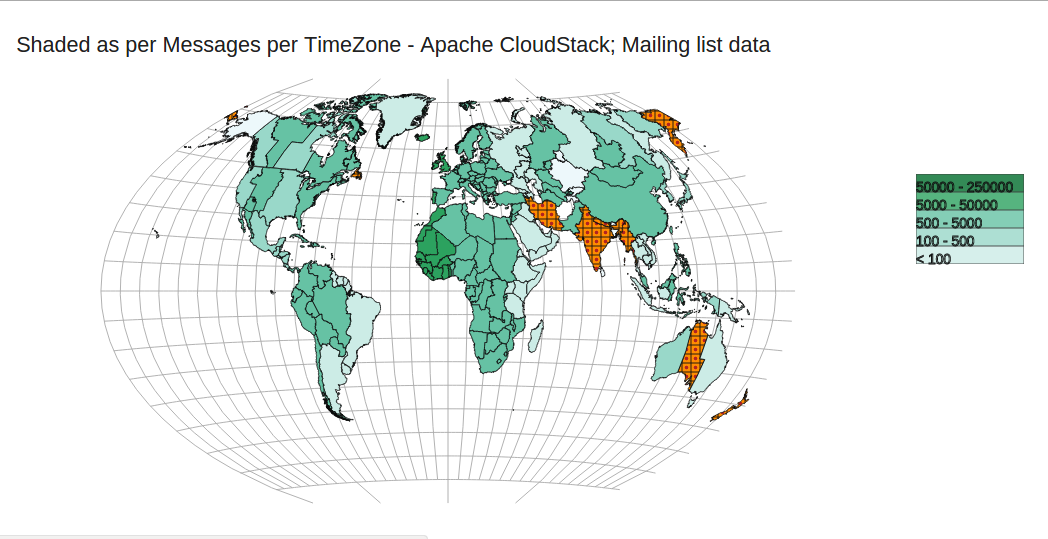
\includegraphics[width=130mm,height=60mm]{image7.png}
\caption{Messages per time zone - Mailing lists}
\label{fig:mgML}
\end{figure}

Figures \ref{fig:div1}, \ref{fig:div2} and \ref{fig:div3} are maps which are shaded with different parameters and the aim here was to try and find a norm or trend that existed for each of the projects.

\begin{figure}[H]
\centering
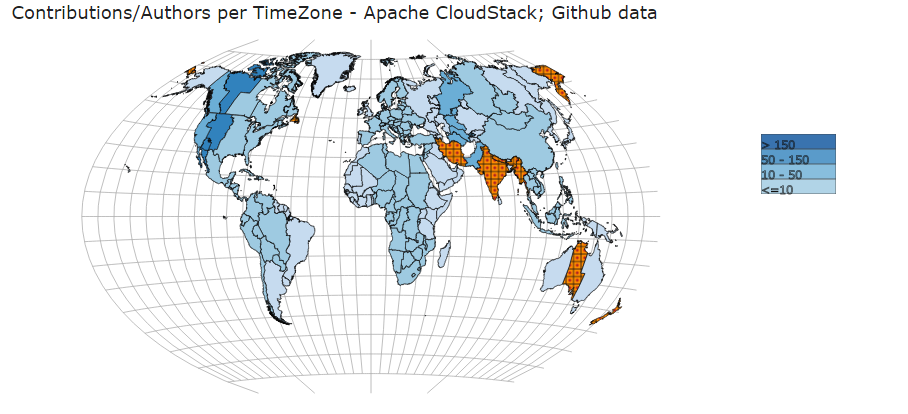
\includegraphics[width=130mm,height=60mm]{image8.PNG}
\caption{Contributions/Author per time zone - Github}
\label{fig:div1}
\end{figure}

\begin{figure}[H]
\centering
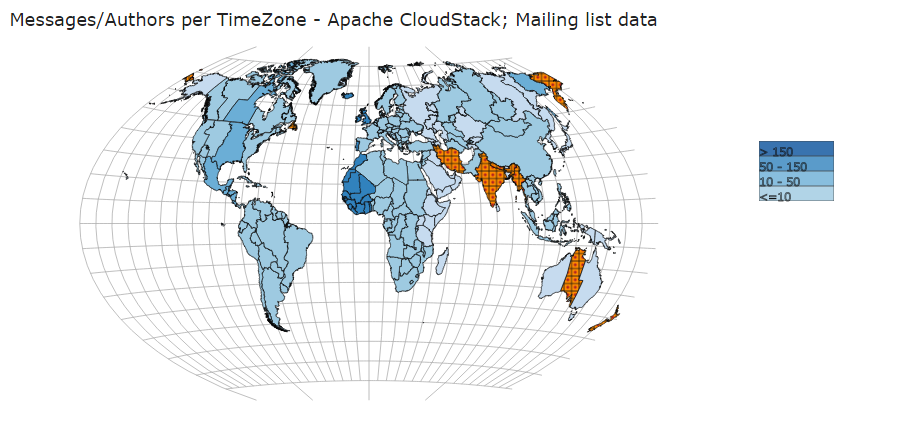
\includegraphics[width=130mm,height=60mm]{image9.PNG}
\caption{Messages/Author per time zone - Mailing lists}
\label{fig:div2}
\end{figure}

\begin{figure}[H]
\centering
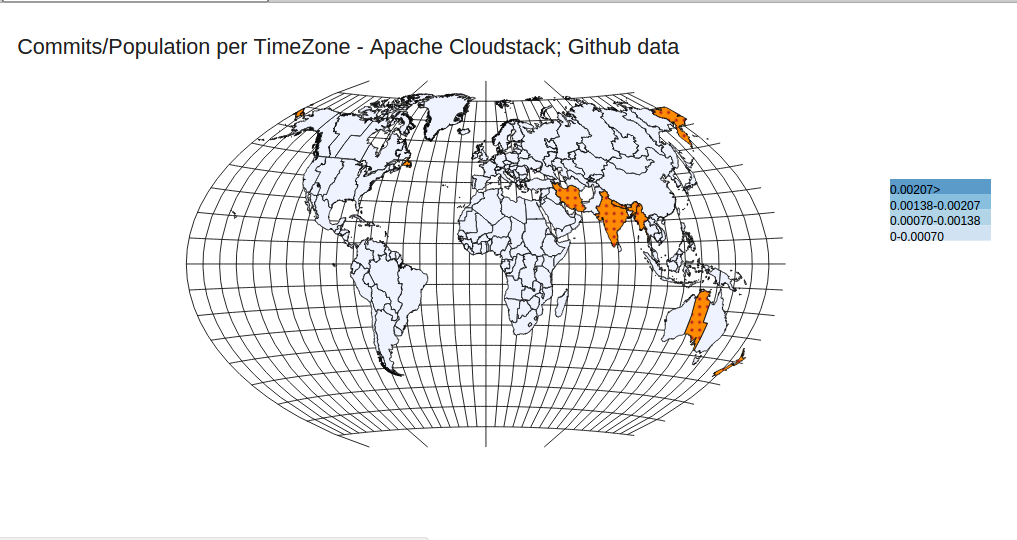
\includegraphics[width=130mm,height=60mm]{image10.png}
\caption{Commits/Population per time zone - Github}
\label{fig:div3}
\end{figure}

\chapter{Evaluation}
In order to gauge the quality and impact of the visualizations, a focus group study was conducted. Focus group sessions are an effective qualitative research method, the main aim of which is to allow the participants to express their point of views and give researchers valuable feedback \cite{villard}.  Focus groups are used to gather information for discovery, benchmarking, evaluating, verifying perceptions, feelings, opinions and thoughts \cite{patton1990}. Focus groups are most productive when used to determine information on new proposals or solutions, determine the strengths and weaknesses of a solution, assessing whether a solution is working and in the evaluation or success of a concept \cite{greenbaum1993}.

\section{Participants}
Six participants over the age of 18 were recruited through the Oregon State University engineering mailing lists by sending out recruitment emails and participant's word of mouth. Table 1 gives an overview of participant demographics. All the participants had some sort of prior experience with software development and have worked with data visualizations at some level. They were made to sign the consent forms before the session and were asked permission to be recorded. Notes were taken and the audio part was transcribed by the researcher.

\begin{table}
\centering
\begin{tabular}{ |p{3cm}||p{5cm}|p{3cm}|p{3cm}|  }
 \hline
Participant Code Name & Degree and Major & Age & Gender\\
 \hline
 A1 & PhD, Computer Science & 25 & Female\\
 A2 & PhD, Computer Science & 27 & Male\\
 A3 & PhD, Botany and Plant Pathology & 30 & Male\\
 A4 & Masters, Computer Science & 25 & Female\\
 A5 & Masters, Computer Science & 24 & Male\\
 A6 & Masters, Electrical and Computer Engineering & 22 & Female\\
 \hline
\end{tabular}
\caption{Participant Demographics}
\label{tab:table1}
\end{table}

\section{Study Session}
The participants were given a nametag with their code names and scenario numbers on arrival. Three of the participants were asked to look at the visualizations done by Bitergia first, and three were given the visualizations done by us first. The goal was to make the participants use both the visualizations and then have a discussion about their effectiveness. The participants were not told beforehand which visualizations they would be handling first. After having completed the tasks with one scenario, the participants then swapped and completed the same tasks with the second set of visualizations. This was a within group study as all participants performed both tasks. This took up 40 minutes of the session. Once done, the participants were led to a discussion session where they were asked some questions with regard to the visualizations. The questions that were posed tried to cover various metrics which would be used to evaluate the visualizations. They were mostly open ended and covered the following topics: a) How close to context were the visualizations, b) Were they easy to understand and use, c) Were meaningful outcomes being drawn, d) How they dealt with missing data etc. All the participants were very enthusiastic and brought out some very interesting points during the course of the discussion. The session lasted for about 2 hours and the collected results were then analysed by means of thematic coding.

\section{Evaluation Metrics}
The evaluation of visualizations has always been subject to a lot of research. One of the oldest research done in this area was by Tufte in 1983 \cite{tufte1983}. Since then lot of researchers have tried their best to formulate a set of guidelines for evaluation, yet no concrete measurable metrics are available today. In 2007, Nico Marrero wrote a paper which spoke about possible metrics derived by various researchers, to evaluate the effectiveness and usability of visualizations \cite{nico2007}. These metrics were divided into three main categories; Mathematical Metrics, User Centric Metrics and Effectiveness Metrics. From this list, 2 metrics were picked under each category to define the usability of the visualizations.

\subsection{Mathematical Metrics}

\begin{enumerate}
\item Reference Context: A visualization needs to provide a context in order to be comprehensible from most viewpoints. This is the number of visible data points in any given visualization with reference to a context \cite{brath1997}.

\item Number of data points and data density: This metric was defined by Tufte when he assumed that the more the amount of data made available per square centimeter of screen size, the more effective is the visualization. The number of data points here mean the discrete number of data sets/values present on the screen at any point and data density is the number of points/pixels on the screen excluding the borders and menu options. It is said that visualizations which cannot show atleast 500 data points, are not found to effective \cite{brath1997}. But this is not a fixed lower bound and can vary depending on the use of the visualization. The same goes for the upper bound; there could be visualizations which have around 100,000 data points and be considered effective and there could be visualizations with just 3000 data points and be deemed complex \cite{brath1997}.
\end{enumerate}

Though these two metrics were mathematical in nature, Nico pointed that as they missed the human element of understanding, one can modify to use these metrics to certify how much the users understand the concepts and can be deemed as user centric metrics in a way as they now consider more of the whole visualization than just the quantitative aspect \cite{nico2007, brath1997}. Hence we used this aspect in our coding sessions to maintain consistency.

\subsection{User Centric Metrics}

\begin{enumerate}
\item Identify Clusters: The ability to group similar data points with similar qualities for better understanding \cite{grins2001}.

\item See all features and data: The visualization should be able to show all of its underlying features and data sets without any occlusion \cite{grins2001}.
\end{enumerate}

\subsection{Effectiveness Metrics}

\begin{enumerate}
\item Dealing with uncertain, missing and dirty data: How effectively can a visualization handle missing and dirty data and bring it across aesthetically to the user \cite{grins2001}.

\item Flexibility of visualization: Visualizations need to have the ability to reach the upper bounds of data density or feature listing without becoming too complex to view \cite{grins2001}.
\end{enumerate}

\section{Code Application}
Each codeset was applied to the chunked transcriptions of the focus study data. Visualization Effectiveness related  codes  were  applied borrowing methods from  grounded theory \cite{corbin2008}, but using pre-­defined codes. Two researchers independently coded all the responses for each scenario and reached a good agreement(Cohen’s  Kappa  coefficient  =  0.718 for scenario A and Cohen’s  Kappa  coefficient  =  0.778 for scenario B).

\chapter{Results}
The questions were all open ended which gave a broad scope. Here scenario A refers to our implementations and scenario B refers to Bitergia's implementation. One thing to be noted is that this was a formative study and was performed to find if the work was heading in the right direction and not to gain consensus or state a solution to be better over the other. The idea was to gather user comments and suggestions for future work.

\section{Task Performance}
The participants were all given around 3-4 questions in each case for both the scenarios and they had to answer them with the help of the visualizations. Upon completion of the tasks, they told the researcher that they had guessed a lot when it came to answering the questions in scenario B. They had done it as they could not take the help of those visualizations to answer the questions completely. This raised questions on the validity of their answers and value of their insights. Below is the summarized result of the solutions given to each question for both scenarios. Find complete responses in the Appendix for these questions.

\subsection{Case 1 response summary}

\begin{enumerate}
\item {\em How does the general trend move towards the number of developers joining each year?}


This question was answered well by using the visualizations from both scenarios by all the participants. The barcharts in both scenarios gave a good idea to find the trends of developers joining each year.


\item {\em Is the number of developers joining a project proportional to the number of developers leaving a project?}


This was one question which had ambiguity when scenario B visualizations were looked at. The participants were not able to clearly demarcate the trend of joining developers vs the trend of leaving developers. However they were all able to answer the questions correctly with scenario A.


\item {\em Do you notice a trend between the conversion and mortality of developers in the open source projects shown here?}


They could not give a concrete answer here as they had to understand a lot more than what was visualized. These answers were all hazy and unclear in scenario B. Scenario A was easy because the there were multiple visualizations and that helped them answer the question.
\end{enumerate}

\subsection{Case 2 response summary}

\begin{enumerate}
\item {\em In any given time zone, does a high number of commits indicate a large number of contributor/author presence?}


For scenario B, three participants said they could not give an answer to the question with the help of the visualization. Three others gave an answer but were not correct. In scenario A, all of them gave correct answers.


\item {\em Can we sense other trends to attribute to the performance levels at any given time zone like lack of Internet, education access etc. from the knowledge that we possess?}


For scenario B, one participant who had knowledge of what countries fell under what time zone tried to give the solution. The other 5 said they could not answer due to lack of this knowledge. For scenario A, all of them answered the question but one of them agreed to have misunderstood the question and gave the wrong answer.


\item{\em Do highly populated regions/time zones have higher contribution rates?}


This question needed knowledge of both, countries in a time zone and their populations. Both of which was lacking in scenario B and required personal knowledge. They answered it better using scenario A, though not completely accurately.

\item {\em Do highly populated regions/time zones have higher contributor rates?}


This question needed knowledge of both countries in a time zone and their populations. Both of which was lacking in scenario B and needed personal knowledge. They answered it better using scenario A as both country data and population in the form of shading was shown.


\end{enumerate}

\section{Focus Group Data Analysis}
\begin{enumerate}
\item \textbf{Were you able to answer all the questions in both scenarios with the help of the visualizations?}

All the participants found scenario B to be a little low on information. They found scenario A to be easier to grasp and make sense of in most cases. They found the case1 i.e., age of developers relatively easy to interpret in both scenarios but the case2 i.e., where do developers work part was difficult in scenario B as they weren't sure what to make of the number -10,-5,0,5,10 in the x axis. Most participants agreed to have guessed a lot of the answers for the scenario B questions as they had a tough time analysing and tying back the questions to the visualizations.
As part of the coding, both researchers found that the participants felt a high reference of context with regard to the visualizations in scenario A with 5 of them making almost direct comments with this regard.

\textbf{Reference Context}

{\em \say{Scenario A was much better atleast to interpret.I was able to find all that I needed from it.}}- A5

\item \textbf{Were the visualizations confusing to understand or seem impractical at any point?}

The participants had one major issue here, they found the axis on both visualizations in scenario B hard to decipher. Also the case1 visualization gave absolute numbers but that is in no way an entity to predict future structuring of a project as they would not know who is leaving and who is staying. Also the case2 visualization issue was that they had no idea how to make sense of the time zone data as most of them did not know which country fell where. They liked how visualization in scenario A played with the colors and was intuitive which helped them as they did not have to tie back the data to the axis all the time. The researchers were found a good mix of reference to context and see all features and data coding metric fit in here with both of them showing up 4 times in the case of scenario A and once for scenario B.

\textbf{See all the features and data}

{\em \say{Ah! Confusion no. I felt like the scenario A, the visualization was a lot more intuitive, the use of colors also helped a lot.}} - A4

{\em \say{I felt like scenario A was a lot more interactive like you could see little labels popup or something like that so I feel like that gives you a lot more information than just the visualization itself.}} - A2

\item \textbf{How effectively did the visualizations handle missing datasets? Were you able to find the missing/dirty data points easily?}

The one thing which came out unanimously was the fact that the orange and dot pattern stood and that helped them know if there was missing/ unavailable data. One participant went on to further explain that in scenario B there was no way one can know if a certain country's data is not available and countries with half time zones are assumed to be clumped with other time zone data. But this was easily answerable in scenario A and it segregated missing data, half time zone data and clean data very well. They did point out that the knowledge of a country's population is personal and it would have been nice to view this on the map somehow as well.All 6 participants made direct response to the feature of handling dirty data. We also coded see all features and data in a few responses.

\textbf{Dealing with uncertain, missing or dirty data}

{\em \say{While scenario A, its very clearly said as you have that orange color with dots saying its missing and that's a good way of saying we don't have data there.}} - A2

\item \textbf{Can we predict future structure of open source projects using the visualizations in either scenario?}

Developer mortality rate very useful visualization as it showed the joining and leaving numbers very well. Also developer turnover visualization gave insight on how many joined the project which can help gauge the interest in a project. Scenario A shows dynamics of a project over scenario B which showed numbers and is not of a lot of interest to them. One participant felt that both scenarios had something to offer with A being on the higher end, but if they were to be combined and viewed that would add a lot of interesting facts maybe. Identifying data clusters was a high preference code with 5 participants reply close to it. Reference to context was a close second place with a frequency of 4 codes.

\item \textbf{Describe the effectiveness of both scenarios in attaining a meaningful outcome as a researcher}

They felt a useful visualization should be able to handle the data very efficiently and use metrics correctly to show multiple data points, both of which were highly available in scenario A visualizations. The fact that there were multiple graphs in scenario A as compared to scenario B pointed out a lot of things to them as different data points were all brought out together and it showed beautiful trends. Again a participant added, a visualization can only be effective when it can serve the purpose of answering the question being asked. Data density, reference to context and see all features and data were the codes applied to most responses with each of them appearing 4 times.

\textbf{Data Density}

{\em \say{It is always important to think about user space whenever displaying visualizations, how does it fit together, how all the data shows up and fits together in that space, how the colors interact with each other and I think the scenario A did a lot better there and did a very good job.}} - A3

\item \textbf{Would adding more data points clutter the visualizations or add to its flexibility?}

Most participants felt that the map visualizations had a lot of potential to show a lot more data by making use of different encodings. One suggested use of colors for one dataset and thickness of border lines for another dataset. Another suggested the use of layering on the maps and clickable countries to add another visualization with more specific data. One participant felt the traditional approach of using barcharts was of less/no use when it came to showing geographic data and the maps worked in this case for them. Most responses spoke about the flexible nature of the visualizations with a frequency of 4.

\textbf{Flexibility of visualizations}

{\em \say{You can use colors for commit frequency and other metric you can show with thickness like internet bandwidth in countries, so nothing overlaps, the map visualizations can handle this well.}} - A1
\end{enumerate}
\section{Metric Frequency for each Scenario}


The table \ref{tab:freq} gives an insight on how both the visualizations stood when it came to evaluating them with the metrics. Scenario A was highly appreciated for its ease of use, contextual nature and flexibility, while scenario B had one major issue of being too stagnant and low on information. The visualizations gave little but were not deemed to be ineffectual. The participants were of the opinion that if the scenario B visualizations would be combined with scenario A visualizations then they might probably add some value to a researcher's quest.

\begin{table}[H]
\centering
\begin{tabular}{ |p{5cm}|p{3cm}|p{3cm}|  }
 \hline
Metric & Scenario A & Scenario B\\
 \hline
 Reference Context & 23 & 5\\ \hline
 See all features and data & 14 & 1\\ \hline
 Flexibility of visualization & 6 & 0\\ \hline
 Dealing with dirty, missing and incorrect data & 8 & 0\\ \hline
 Data density & 3 & 0\\ \hline
 Identify Clusters & 15 & 2\\ \hline
 No code applied & 9 & 42\\ 
 \hline
\end{tabular}
\caption{Evaluation Metric Frequency for each Scenario}
\label{tab:freq}
\end{table}

\begin{figure}[!ht]
\centering
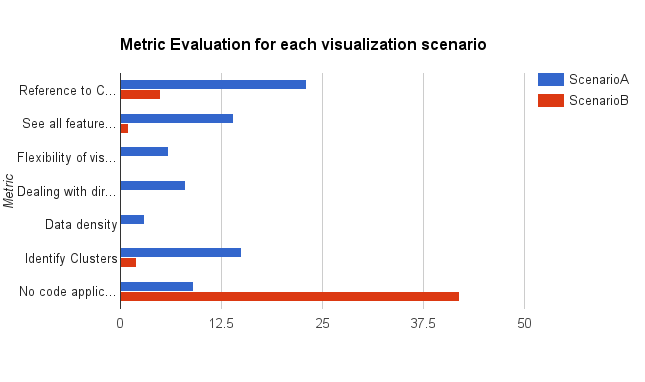
\includegraphics[width=140mm,height=70mm]{metric.png}
\caption{Metric Evaluation}
\end{figure}

\chapter{Threats to Validity}
\section{Internal Threats}
\begin{enumerate} 
\item In our study, all participants had to answer the same set of questions for both scenario A and scenario B. This creates a confound effect as it is possible that one scenario was actually a lot more effective to answer the questions over the other. So this could lead to a set of participants using the previous scenario's knowledge to answer for the new scenario. This effect was reduced by alternating the order of scenarios given to the participants.
\end{enumerate}

\section{External Threats}
\begin{enumerate}
\item The participants of the study might not be representative of the actual target population.
\item The tasks chosen might not be completely representative of the tasks looked at by researchers.
\end{enumerate}

\section{Reliability Threats}
\begin{enumerate}
\item As participants might not be representative of the target population, the results/findings might not be replicable in real world.
\item In cases where the participants guessed the answers for either scenario would lead to reliability issues.
\item As the study was conducted by the researcher alone the possibility of missing out on a few notes/comments from the participants or misinterpretation of the data is possible.
\end{enumerate}


\chapter{Summary}
A large number of developers contribute to open source projects from all over the world and it becomes important to understand their working behaviour to gauge their interest in the project and the growth of the project. Visualizations add a lot of drama to a dataset making it reflect things that the naked eye can't always see. In our case the aim was to make visualizations which would help understand the way developers work/contribute to an open source project to infer the future scope of these projects. As stated by one of the user study participants, \say{It all
depends on what the message is and how it can be conveyed effectively.} Both visualizations had their own shares of advantages and disadvantages, but scenario A stood out plainly because it gave out the message clearly and in multiple ways. Scenario B was not thrown out by our participants, they felt it had potential too, if modified and looked at, along with the visualizations in Scenario A. Having said this there is room for improvement in the Scenario A implementations as well, as a wide variety of suggestions were obtained from the participants. Another point to be noted is, due to the small size of the group there is scope for conducting further studies to get more feedback.

\bibliographystyle{unsrt}
\bibliography{thesis}

\begin{appendices}
\chapter{Task Responses}

Scenario A responses

Case1

1.How does the general trend move towards the number of developers joining each year?

\begin{table}[H]
\begin{tabular}{ |p{2cm}|p{12cm}| }
 \hline
 A1 & Apache CloudStack: The project probably started in 2010 (no established developers), and with a sizeable community (40-50 people) . Perhaps it was outsourced then. And then, there was an increase in the number of developers joining between 2010-2013. Decreased in 2014 and dropped in 2015. The ratio of new to established developers also followed a similar trend until 2012, and dropped between 2013-2015.\\
 \hline
 A2 & It grows every year with a taper in 2015. Probably because the year isn't over yet.\\ \hline
 A3 & It was increasing, but now it's static\\ \hline
 A4 & There has been an increase in developers joining the project till 2013, but the numbers start to decline starting 2014:Apache Cloudstack\\ \hline
 A5 & The trend moves on pretty slow, and slowly increases until it reaches maturity period. After that either new technology may take over the existing or the existing technology would be stagnated at certain point\\ \hline
 A6 & In most cases until 2014 it increased but there was decrease in number of developers in 2015.\\
 \hline
\end{tabular}
\caption{Task Response 1 - scenario A, case1}
\label{tab:table1}
\end{table}

2.Is the number of developers joining a project proportional to the number of developers leaving a project?

\begin{table}[H]
\begin{tabular}{ |p{2cm}|p{12cm}| }
 \hline
 A1 & Yes\\
 \hline
 A2 & No. The number of developers leaving does decrease over time, while the number of incoming developers increases\\ \hline
 A3 & No. There appear to be more leaving the project after a few years\\ \hline
 A4 & They are somewhat proportional. The number of people that decide to stay are very low compared to the number of people that joined.\\ \hline
 A5 & No, the number of developers joining the project is not proportional to once who are leaving. It actually depends on the type of project, popularity and whether it satisfies the interest of the ever-changing demands\\ \hline
 A6 & Yes\\
 \hline
\end{tabular}
\caption{Task Response 2 - scenario A, case1}
\label{tab:table2}
\end{table}


3. Do you notice a trend between the conversion and mortality of developers in the open source projects shown here?

\begin{table}[H]
\begin{tabular}{ |p{2cm}|p{12cm}| }
 \hline
 A1 & Both rise, until in 2014 it stabilizes. More people stayed, and less newer people joined.\\
 \hline
 A2 & The conversion rate seems to increase while the mortality rate decreases.\\ \hline
 A3 & Yes. As the project grows, more of the early developers are gone.\\ \hline
 A4 & The conversion rate seems pretty low compared to the mortality rate.\\ \hline
 A5 & Yes\\ \hline
 A6 & In most cases mortality rate decreases\\
 \hline
\end{tabular}
\caption{Task Response 3 - scenario A, case1}
\label{tab:table3}
\end{table}

Case2

1.In any given time zone, does a high number of commits indicate a large number of contributor/author presence?

\begin{table}[H]
\begin{tabular}{ |p{2cm}|p{12cm}| }
 \hline
 A1 & No.\\
 \hline
 A2 & Yes. I can see the number of authors and the number of commits, so I can see a correlation between the two.\\ \hline
 A3 & Yes\\ \hline
 A4 & It depends on the time that people prefer to make their contributions. The evening for one country might be the morning time for another country and people might be making contributions in both countries because come people might be making contributions at work and other might be making contributions after work.\\ \hline
 A5 & Yes\\ \hline
 A6 & Yes.\\
 \hline
\end{tabular}
\caption{Task Response 1 - scenario A, case2}
\label{tab:table11}
\end{table}

2.Can we sense other trends to attribute to the performance levels at any given time zone like lack of Internet, education access etc. from the knowledge that we possess?

\begin{table}[H]
\begin{tabular}{ |p{2cm}|p{12cm}| }
 \hline
 A1 & No, Africa for example, has a high number commits per time zone.\\
 \hline
 A2 & Time zones clump the world longitudinally. Most of Africa is on the same time one as Western Europe. Same applies for South America with North America. The only place when such a trend can be seen is Asia, where one would expect a higher number of contributors due to a higher population.\\ \hline
 A3 & No\\ \hline
 A4 & The lack of internet and education are very big factors. Even if you have a large population, and the population is not very educated then the contribution rates are going to be low.\\ \hline
 A5 & No.\\ \hline
 A6 & Yes.\\
 \hline
\end{tabular}
\caption{Task Response 2 - scenario A, case2}
\label{tab:table12}
\end{table}

3.Do highly populated regions/time zones have higher contribution rates?

\begin{table}[H]
\begin{tabular}{ |p{2cm}|p{12cm}| }
 \hline
 A1 & No, Africa for example, has a high number commits per time zone.\\
 \hline
 A2 & Time zones clump the world longitudinally. Most of Africa is on the same time one as Western Europe. Same applies for South America with North America. The only place when such a trend can be seen is Asia, where one would expect a higher number of contributors due to a higher population.\\ \hline
 A3 & Yes.\\ \hline
 A4 & The lack of internet and education are very big factors. Even if you have a large population, and the population is not very educated then the contribution rates are going to be low.\\ \hline
 A5 & No.\\ \hline
 A6 & Yes.\\
 \hline
\end{tabular}
\caption{Task Response 3 - scenario A, case2}
\label{tab:table13}
\end{table}

4.Do highly populated regions/time zones have higher contributor numbers?

\begin{table}[H]
\begin{tabular}{ |p{2cm}|p{12cm}| }
 \hline
 A1 & No, again South Asia or China does not show that trend.\\
 \hline
 A2 & No. Same answer as previous.\\ \hline
 A3 & Yes.\\ \hline
 A4 & No.\\ \hline
 A5 & May be, again it depend on quality of education,awareness, technology affecting the people over there.\\ \hline
 A6 & Yes.\\
 \hline
\end{tabular}
\caption{Task Response 4 - scenario A, case2}
\label{tab:table14}
\end{table}

Scenario B responses

Case1

1.How does the general trend move towards the number of developers joining each year?	

\begin{table}[H]
\begin{tabular}{ |p{2cm}|p{12cm}| }
 \hline
 A1 & Increases. However, there is an increase in the number of developers with lesser experience.\\
 \hline
 A2 & It grows. The labels on the X axis are hard to read
\\ \hline
 A3 & Yes.\\ \hline
 A4 & More developers are joining later in the year.\\ \hline
 A5 & It is gradual and slow, and awareness about type of technology which interest may interest developer and organisation.\\ \hline
 A6 & 10.\\
 \hline
\end{tabular}
\caption{Task Response 1 - scenario B, case1}
\label{tab:table21}
\end{table}

2.Is the number of developers joining a project proportional to the number of developers leaving a project?	

\begin{table}[H]
\begin{tabular}{ |p{2cm}|p{12cm}| }
 \hline
 A1 & Yes, the leaving happens in the top part of the graphs (higher experience) and the joining happens in the lower part. Also, these are regular triangles, with almost similar area. Hence the number of developers seems to remain the same, while the average experience shifts to the bottom, year on year.\\
 \hline
 A2 & I cannot say. I only have absolute numbers, and the visualization does not show people leaving or entering the project.\\ \hline
 A3 & This is not clear. I'll say.... No?\\ \hline
 A4 & In my opinion the number of people joining a project is greater than the number of people leaving the project. Because of this the number of people at any time working on a project has increased consistently over the years.\\ \hline
 A5 & No, it depends on the type of technology, interest of an organisation and developer. More likely developers interest plays an important role I feel.\\ \hline
 A6 & In most scenarios it is proportional..\\
 \hline
\end{tabular}
\caption{Task Response 2 - scenario B, case1}
\label{tab:table22}
\end{table}

3.Do you notice a trend between the conversion and mortality of developers in the open source projects shown here?

\begin{table}[H]
\begin{tabular}{ |p{2cm}|p{12cm}| }
 \hline
 A1 & Conversion happened in the developers with lesser experience, and increasing number of more experienced developers left.\\
 \hline
 A2 & No\\ \hline
 A3 & Not particularly.\\ \hline
 A4 & Not sure.\\ \hline
 A5 & --\\ \hline
 A6 & Yes, in general they tend to increase.\\
 \hline
\end{tabular}
\caption{Task Response 3 - scenario B, case1}
\label{tab:table23}
\end{table}

CAse2

1.In any given time zone, does a high number of commits indicate a large number of contributor/author presence?	

\begin{table}[H]
\begin{tabular}{ |p{2cm}|p{12cm}| }
 \hline
 A1 & Does not show it.\\
 \hline
 A2 & No really. It could be just one very active developer in that region\\ \hline
 A3 & Assuming x is time zone, I don't have enough information since y is messages.\\ \hline
 A4 & Yes.\\ \hline
 A5 & Yes.\\ \hline
 A6 & Yes.\\
 \hline
\end{tabular}
\caption{Task Response 1 - scenario B, case2}
\label{tab:table31}
\end{table}

2.Can we sense other trends to attribute to the performance levels at any given time zone like lack of Internet, education access etc. from the knowledge that we possess?	

\begin{table}[H]
\begin{tabular}{ |p{2cm}|p{12cm}| }
 \hline
 A1 & Does not show it.\\
 \hline
 A2 & Well, most commits are from the UTC to UTC-2 which contains western Europe and around UTC-5, which contains North America. Some of the time zones contain only water, so it's natural that no developers live there. Also, good parts of Africa are also under the same time zone as Europe. So it is very difficult to distinguish between these two time zones. Also, the same applies for South America\\ \hline
 A3 & No.\\ \hline
 A4 & Some people may not have internet access in their houses so all their contribution may happen at work, but it does depend on the country that the developer is from.\\ \hline
 A5 & Yes.\\ \hline
 A6 & yes several other factors tend to influence the performance levels.\\
 \hline
\end{tabular}
\caption{Task Response 2 - scenario B, case2}
\label{tab:table32}
\end{table}

3.Do highly populated regions/time zones have higher contribution rates?	

\begin{table}[H]
\begin{tabular}{ |p{2cm}|p{12cm}| }
 \hline
 A1 & Does not show it.\\ \hline
 A2 & No. UTC+10 and around does contain India and China, which are heavily populated. However, the number of messages does not spike there.\\ \hline
 A3 & Again, assuming x is time zone, I don't have enough data.\\ \hline
 A4 & Just because the population is high does not mean that the everyone in that country have the knowledge required to make contributions.\\ \hline
 A5 & Depends on the knowledge level, and technology trend in that time zone. People would contribute to that technology which is more likely used in that time zone.\\ \hline
 A6 & Yes.\\
 \hline
\end{tabular}
\caption{Task Response 3 - scenario B, case2}
\label{tab:table33}
\end{table}

4.Do highly populated regions/time zones have higher contributor numbers?

\begin{table}[H]
\begin{tabular}{ |p{2cm}|p{12cm}| }
 \hline
 A1 & Does not show it.\\
 \hline
 A2 & Again no. Same answer as above.
\\ \hline
 A3 & I don't have enough data to answer that question.\\ \hline
 A4 & My answer is similar to the previous one.\\ \hline
 A5 & Again Depends, on the knowledge level in that time zone.\\ \hline
 A6 & Yes.\\
 \hline
\end{tabular}
\caption{Task Response 4 - scenario B, case2}
\label{tab:table34}
\end{table}

\end{appendices}

\end{document}